\section{Descrição da estrutura}

A seguir, são apresentadas as dimensões e características da estrutura do robô.

\begin{figure}[htb]
  \caption{\label{fig:structure-down} Visão inferior do robô}

  \begin{center}
    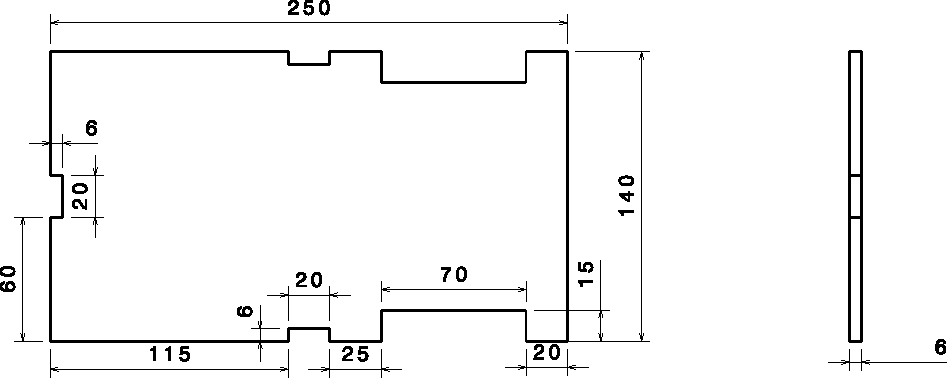
\includegraphics[scale=0.525,page=1]{../img/structure.pdf}
  \end{center}

  \legend{Fonte: Elaborado pelos autores.}
\end{figure}

\begin{figure}[htb]
  \caption{\label{fig:structure-side} Visão lateral do robô}

  \begin{center}
    \includegraphics[scale=0.525,page=2]{../img/structure.pdf}
  \end{center}

  \legend{Fonte: Elaborado pelos autores.}
\end{figure}

\begin{figure}[htb]
  \caption{\label{fig:structure-back} Visão traseira do robô}

  \begin{center}
    \includegraphics[scale=0.525,page=3]{../img/structure.pdf}
  \end{center}

  \legend{Fonte: Elaborado pelos autores.}
\end{figure}

\begin{figure}[htb]
  \caption{\label{fig:structure-front} Visão frontal do robô}

  \begin{center}
    \includegraphics[scale=0.525,page=4]{../img/structure.pdf}
  \end{center}

  \legend{Fonte: Elaborado pelos autores.}
\end{figure}

\begin{figure}[htb]
  \caption{\label{fig:structure-up} Visão superior do robô}

  \begin{center}
    \includegraphics[scale=0.525,page=5]{../img/structure.pdf}
  \end{center}

  \legend{Fonte: Elaborado pelos autores.}
\end{figure}

\begin{figure}[htb]
  \caption{\label{fig:structure-iso} Visão isométrica do robô}

  \begin{center}
    \includegraphics[scale=0.525,page=6]{../img/structure.pdf}
  \end{center}

  \legend{Fonte: Elaborado pelos autores.}
\end{figure}
